\documentclass[border=10pt]{standalone}
\usepackage{tkz-graph}
\GraphInit[vstyle = Shade]
\tikzset{
  LabelStyle/.style = { rectangle, rounded corners, draw,
                        minimum width = 2em, fill = yellow!50,
                        text = red, font = \bfseries },
  VertexStyle/.append style = { inner sep=5pt,
                                font = \Large\bfseries},
  EdgeStyle/.append style = {->, bend left} }
\thispagestyle{empty}
\begin{document}
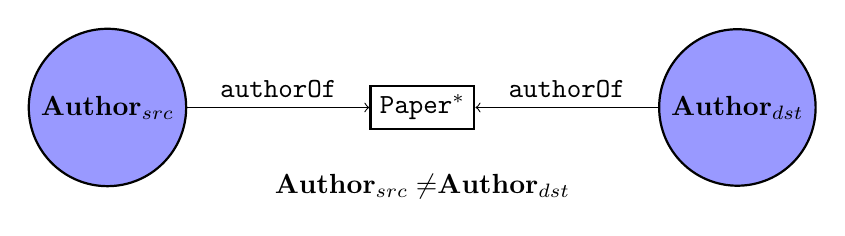
\begin{tikzpicture}
  \node[circle,thick,draw,fill=blue!40] (src) {\textbf{Author}$_{src}$};
  \node[thick,draw] at (4,0) (mid) {\texttt{Paper}$^*$};
  \node at (4,-1) {\textbf{Author}$_{src}\neq$\textbf{Author}$_{dst}$};
  \node[circle,thick,draw,fill=blue!40] at (8,0) (dst) {\textbf{Author}$_{dst}$};
  \path[->] (src) edge node [above,midway] {\texttt{authorOf}} (mid);
  \path[->] (dst) edge node [above,midway] {\texttt{authorOf}} (mid);
\end{tikzpicture}
\end{document}